\documentclass[12pt, a4paper, oneside]{ctexbook}
\usepackage{amsmath, amsthm, amssymb, bm, graphicx, hyperref, mathrsfs, verbatim}
\usepackage{makecell}
\usepackage{longtable}
\usepackage{xcolor}
\usepackage{tcolorbox}
\usepackage{soul}
\usepackage{adjustbox}
\usepackage{tcolorbox}
\usepackage{enumerate}
\usepackage{pdfpages}
\usepackage{float}
\usepackage{colortbl}
\usepackage{tabularx}
\usepackage{multirow}
\usepackage{pgfplots}
\usepackage{underscore}
\usepackage{listings}
\usepackage{minted}
\numberwithin{figure}{section}
\title{{\Huge{\textbf{嵌入式开发}}}}
\author{Boyuan Zhao}
\date{\today}
\linespread{1.5}
\newtheorem{theorem}{定理}[section]
\newtheorem{definition}[theorem]{定义}
\newtheorem{lemma}[theorem]{引理}
\newtheorem{corollary}[theorem]{推论}
\newtheorem{example}[theorem]{例}
\newtheorem{proposition}[theorem]{命题}

\begin{document}

\maketitle

\pagenumbering{roman}
\setcounter{page}{1}

\begin{center}
    \Huge\textbf{前言}
\end{center}~\

临时抱佛脚. 
~\
\begin{flushright}
    \begin{tabular}{c}
        Boyuan Zhao\
        \today
    \end{tabular}
\end{flushright}

\newpage
\pagenumbering{Roman}
\setcounter{page}{1}
\tableofcontents

\newpage
\setcounter{page}{1}
\pagenumbering{arabic}

\chapter{STM32开发}

在这里可以输入笔记的内容. 

\section{STM32的基本知识}

这是笔记的正文部分. 

\clearpage

\chapter{Linux开发}

\section{Linux操作基本指令}

\subsection{目录操作}

\begin{verbatim}
    pwd             # 查看当前目录
    cd ..           # 返回上一层目录
    cd <directory>  # 进入特定目录
    cd ~            # 返回用户主目录

    mkdir <dir_name> # 创建新目录
    rmdir <dir_name> # 删除空目录
    rm -r <dir_name> # 删除非空目录

    mv <old_dir> <new_dir> # 重命名或移动目录
\end{verbatim}

\subsection{文件操作}

\begin{verbatim}
    touch <filename>  # 创建新文件
    ls                # 列出目录内容
    ls -l             # 详细列出目录内容

    # 以下是一个文件权限的示例:
    # -rw-rw-r--. 1 test test  0 Mar 25 01:44 file1
    # drwxr-xr-x. 2 test test  6 Mar 25  2022 Music

    # 用户,组,其他
    # rwx   rwx   rwx
    # r: read, w: write, x: execute

    ls -a             # 列出所有文件,包括隐藏文件
    ls -la            # 详细列出所有文件,包括隐藏文件

    cat <filename>    # 查看文件内容
    rm <filename>     # 删除文件
    mv <old_file> <new_file> # 重命名或移动文件

    cp <src_file> <dest_file>   # 复制文件
    cp -r <src_dir> <dest_dir>  # 复制目录
\end{verbatim}

\subsection{系统命令}

\begin{verbatim}
    su                  # 切换用户
    yum install openssh-server  # 安装 OpenSSH 服务器
    useradd <username>  # 添加新用户
    passwd [username]   # 设置或更改用户的密码
    ps -aux | more      # 查看进程
    kill <process_id>   # 杀死进程
    top                 # 显示系统任务,按q退出
    uptime              # 显示系统运行时间
    # 改变文件权限
    # chmod [ugoa][+-][rwx] <filename>
    # u: owner, g: group, o: other, a: all (ugo)
    # 或者
    # chmod <numeric_permissions> <filename>
    # r:4, w:2, x:1
    find . -name <name> # 在当前目录下查找具有特定名称的文件或目录
    tar -zcvf test1.tar.gz test1/  # 创建gzip压缩包
    tar -zxvf test1.tar.gz  # 解压gzip压缩包
\end{verbatim}

\subsection{网络命令}

\begin{verbatim}
    ifconfig  # 显示网络配置
    ping <domain/ip_address>  # 发送 ICMP 请求以测试网络连接
    netstat -ant  # 显示网络统计信息
\end{verbatim}

\subsection{Vim操作}
\begin{verbatim}
    i:  Enter editing mode, insert at cursor.        # 进入编辑模式,在光标处插入。
    x:  Delete a character.                          # 删除一个字符
    dd: Delete a line.                               # 删除一行
    ndd:Delete n lines.                              # 删除n行
    yy: Copy a line.                                 # 复制一行
    nyy:Copy n lines.                                # 复制n行
    p:  Paste.                                       # 粘贴
    nG: Move cursor to line n.                       # 移动光标到n行
    G:  Move to the last line.                       # 移动到最后一行
    $:  Move to the end of this line.                # 移动到这一行的末尾
    ^:  Move to the start of this line.              # 移动到这一行的开始
    /string: Search for string.                      # 查找string
    ?string: Search for string upwards.              # 向上查找string
    
    Edit vim configuration:
    ~/.vimrc
    set tabstop=4    # 设置tab宽度为4个空格
    set expandtab    # 将tab转化为空格
    \end{verbatim}
\section{Linux基本概念}

\subsection{系统调用}
    
系统调用是操作系统提供的用户程序向操作系统请求服务的接口。在Linux中,它们是用来使进程能够访问硬件设备和操作系统服务的基础。例如,当一个进程需要打开一个文件或者创建一个新进程时,它会执行一个系统调用。这些系统调用的接口在Linux内核中实现,当一个进程需要使用某个系统服务时,它将执行一个特定的系统调用,然后内核将执行所需的服务,然后将结果返回给进程。

\subsection{进程}
    
进程是Linux中的基本执行实体,它包含执行程序所需的所有资源,如CPU时间、内存空间等。每个进程都有一个唯一的进程ID,以及一套完整的系统资源,如打开的文件、挂起的信号、内部状态、优先级等。Linux支持多进程并发执行,因此可以在同一时间运行多个任务。
\begin{figure}[H]
\centering
 \resizebox{0.75\textwidth}{!}{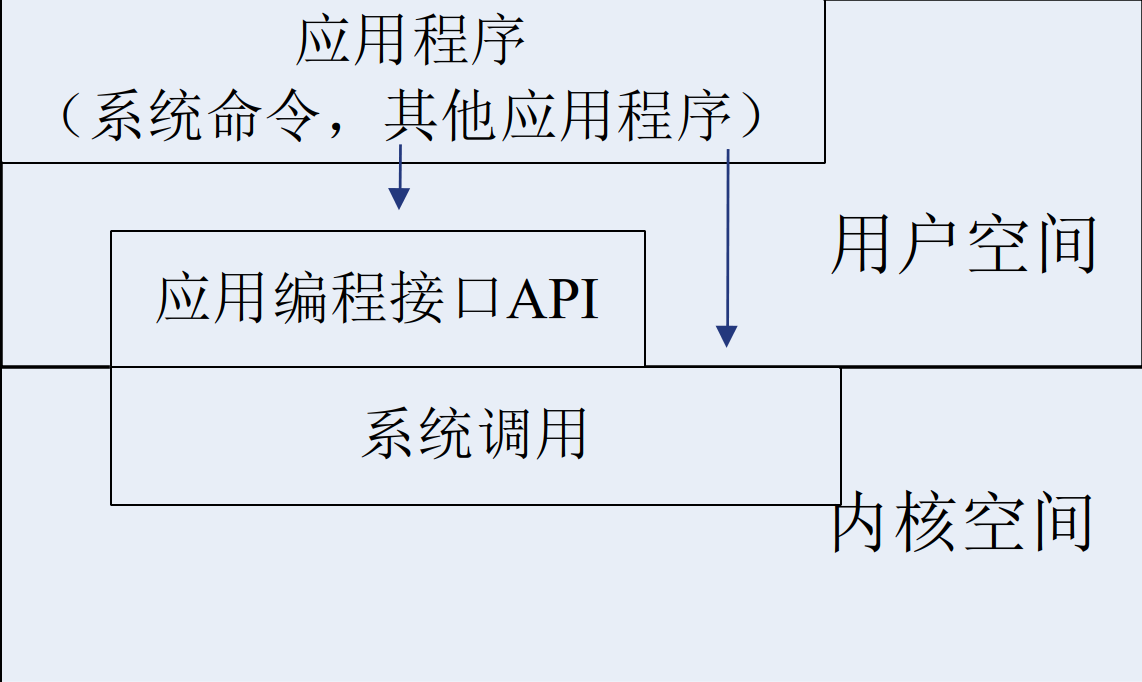
\includegraphics{linux1.png}}
 \caption{}
 \label{}
\end{figure}
\subsection{进程间通信}
    
进程间通信(IPC,Inter-Process Communication)指的是在同一操作系统中运行的不同进程之间传递信息或信号的机制。在Linux系统编程中,常见的IPC机制包括管道、信号、消息队列、共享内存、信号量等。
    
\subsection{线程}
    
线程是程序中的单一顺序控制流程,是操作系统能够进行运算调度的最小单位。它被包含在进程之中,是进程中的实际运作单位。同一进程内的多个线程将共享该进程的资源。多线程能提高程序的并发性,以提高应用程序的响应速度。在Linux中,线程是轻量级的进程,因此也拥有一些类似于进程的属性,但由于线程共享了进程的资源,所以线程之间的切换比进程之间的切换更加高效。

\subsection{Linux应用编程接口API}

Linux应用编程接口(API,Application Programming Interface)是一系列函数和过程,允许创建的应用程序可以访问操作系统的特定功能和资源。Linux API提供了大量的库函数,用于实现各种任务,如文件操作、网络通信、内存管理等。这些库函数在程序调用时,最终都会被映射到具体的系统调用。
    
\subsubsection{请求机制}
    
请求API函数的过程通常包括创建一个包含特定参数的数据结构,然后调用与任务相对应的API函数。API函数会将参数数据结构传递给操作系统内核,内核再执行相应的系统调用。

\subsubsection{标准}
    
Linux API主要遵循两个标准:POSIX和GNU。POSIX(Portable Operating System Interface)是IEEE为了实现软件在UNIX操作系统间的可移植性而制定的一系列API标准。GNU库(Glibc)是GNU项目发布的用于提供系统调用的C库,它基本上遵循POSIX标准,但同时也提供了一些额外的API。
    
\subsubsection{实现方法}
    
Linux API的实现涉及到用户空间和内核空间的交互。当程序调用一个API函数时,该函数会创建一个系统调用,并将控制权交给操作系统。操作系统会切换到内核模式,执行系统调用,然后返回结果,最后再切换回用户模式。
    
\subsection{Linux系统命令}
    
Linux系统命令是在命令行接口(CLI)中执行操作的文本输入。Linux系统提供了大量的系统命令,用于执行各种任务,如文件操作(如ls、cd、mv等)、系统监控(如top、ps等)、网络工具(如ping、netstat等)等。在Linux系统编程中,可以通过系统调用来执行这些系统命令。每个系统命令都有一系列的选项和参数,可以用来定制命令的行为。

\section{文件及文件描述符}

\subsection{文件}

在Linux系统中,几乎所有的事物都可以被视为文件。这些包括硬件设备、目录,甚至是网络通信,它们在Linux中都可以被当作文件来处理。文件是一个包含数据的容器,数据可以以任何格式存储在文件中。文件包含两部分信息:用户数据和元数据。用户数据是文件的主体部分,元数据则包含了关于文件的信息,如文件的大小、创建和修改时间、所有者和权限等。

\textbf{Linux文件类型:普通文件、目录文件、链接文件、设备文件}

\subsection{文件描述符}

文件描述符是一个用于访问文件或者其他输入/输出资源,如管道或网络套接字的非负整数。在Linux系统中,文件描述符是在进程中创建的,并在进程的生命周期内使用。它们是由内核自动分配的,并且总是返回最小的未使用的文件描述符。例如,当进程打开一个现有文件或者创建一个新文件时,操作系统将返回一个文件描述符以供进程在后续操作中使用。

在每个进程启动时,它都会有三个已经打开的文件描述符。标准输入(STDIN)的文件描述符是0,标准输出(STDOUT)的文件描述符是1,以及标准错误(STDERR)的文件描述符是2。这些文件描述符通常连接到用户的终端。

在Linux系统编程中,有多种系统调用用于操作文件描述符,如open, read, write, close等。

\section{底层文件I/O操作}

\subsection{打开文件}

在Linux中,可以使用系统调用 open() 打开一个文件。该函数需要文件名和打开模式作为参数,如只读、只写或读写等。如果操作成功,open() 将返回一个文件描述符,它是一个小的非负整数,可以在程序中用于引用该打开的文件。如果出错,open() 将返回-1。

\begin{verbatim}
    #include <fcntl.h>
    int open(const char *path, int flags);
    int open(const char *path, int flags, mode_t mode);
\end{verbatim}

\subsection{读取文件}

读取文件是通过 read() 系统调用完成的。该函数需要文件描述符、数据缓冲区的地址和要读取的字节数作为参数。read() 返回实际读取的字节数,如果已经到达文件末尾,那么返回0,如果出现错误则返回-1。

\begin{verbatim}
    #include <unistd.h>
    ssize_t read(int fd, void *buf, size_t count);
\end{verbatim}

\subsection{写入文件}

向文件中写入数据是通过 write() 系统调用完成的。该函数需要文件描述符、数据缓冲区的地址和要写入的字节数作为参数。write() 返回实际写入的字节数,如果出现错误则返回-1。

\begin{verbatim}
    #include <unistd.h>
    ssize_t write(int fd, const void *buf, size_t count);
\end{verbatim}

\subsection{关闭文件}

关闭文件是通过 close() 系统调用完成的。该函数需要文件描述符作为参数,如果关闭操作成功,那么返回0,如果出现错误则返回-1。

\begin{verbatim}
    #include <unistd.h>
    int close(int fd);
\end{verbatim}

\subsection{定位文件读写位置}

通过 lseek() 系统调用可以在文件中改变当前的读写位置。该函数需要文件描述符、偏移量和基准点作为参数。如果操作成功,返回新的读写位置,如果出现错误则返回-1。

\begin{verbatim}
    #include <unistd.h>
    off_t lseek(int fd, off_t offset, int whence);
\end{verbatim}


\subsection{文件锁}

在Linux中,可以使用文件锁(File Lock)来实现对文件的互斥访问。文件锁分为共享锁(Shared Lock)和独占锁(Exclusive Lock),用于控制对文件的读写操作。

\subsubsection{设置文件锁}

文件锁的设置使用 fcntl() 系统调用。通过设置 F_SETLK 或 F_SETLKW 命令,可以获取或释放文件锁。

\begin{verbatim}
#include <fcntl.h>
int fcntl(int fd, int cmd, struct flock *lock);
\end{verbatim}

其中,fd 是文件描述符,cmd 是命令,lock 是指向 struct flock 结构的指针,该结构定义了文件锁的类型和位置。在设置文件锁时,需要设置以下字段:

\begin{itemize}
\item l_type:锁的类型,可以是 F_RDLCK(共享锁)或 F_WRLCK(独占锁)。
\item l_whence:偏移量的基准点,可以是 SEEK_SET、SEEK_CUR 或 SEEK_END。
\item l_start:锁定区域的起始偏移量。
\item l_len:锁定区域的长度。
\end{itemize}

\subsubsection{测试文件锁}

文件锁的测试使用 fcntl() 系统调用。通过设置 F_GETLK 命令,可以检测给定的锁是否会阻塞。

\begin{verbatim}
#include <fcntl.h>
int fcntl(int fd, int cmd, struct flock *lock);
\end{verbatim}

其中,fd 是文件描述符,cmd 是命令,lock 是指向 struct flock 结构的指针。在测试文件锁时,需要设置以下字段:

\begin{itemize}
\item l_type:锁的类型,可以是 F_RDLCK(共享锁)或 F_WRLCK(独占锁)。
\item l_whence:偏移量的基准点,可以是 SEEK_SET、SEEK_CUR 或 SEEK_END。
\item l_start:锁定区域的起始偏移量。
\item l_len:锁定区域的长度。
\end{itemize}

\subsubsection{释放文件锁}

文件锁的释放使用 fcntl() 系统调用。通过设置 F_SETLK 命令,并将锁的类型设置为 F_UNLCK,可以释放文件锁。

\begin{verbatim}
#include <fcntl.h>
int fcntl(int fd, int cmd, struct flock *lock);
\end{verbatim}

其中,fd 是文件描述符,cmd 是命令,lock 是指向 struct flock 结构的指针。在释放文件锁时,需要设置以下字段:

\begin{itemize}
\item l_type:锁的类型,设置为 F_UNLCK。
\item l_whence:偏移量的基准点,可以是 SEEK_SET、SEEK_CUR 或 SEEK_END。
\item l_start:锁定区域的起始偏移量。
\item l_len:锁定区域的长度。
\end{itemize}

文件锁对于控制多个进程对同一文件的并发访问非常有用,可以防止数据损坏或不一致性。

\section{标准I/O编程}

\subsection{概述}

Linux标准I/O库提供了一组函数,用于读写流,这些函数比系统调用更易于使用。在C语言中,标准I/O库被包含在stdio.h头文件中。

\subsection{标准I/O函数}

\subsubsection{读函数}

\begin{itemize}
    \item \texttt{fgetc}: 从流中获取下一个字符。
    \item \texttt{fgets}: 从流中获取下一行。
    \item \texttt{fread}: 从流中读取数据。
\end{itemize}

\subsubsection{写函数}

\begin{itemize}
    \item \texttt{fputc}: 向流中写入一个字符。
    \item \texttt{fputs}: 向流中写入一个字符串。
    \item \texttt{fwrite}: 向流中写入数据。
\end{itemize}

\subsection{缓冲}

标准I/O库使用缓冲来减少读写操作的数量。这意味着当你调用一个写函数时,数据可能不会立即写入磁盘,而是存储在缓冲区中,等待缓冲区满了或者你显式地刷新缓冲区。

标准I/O提供3种类型的缓冲存储:

\subsubsection{全缓冲}

在这种阻塞I/O模型中,填满标准I/O缓存后才进行实际I/O操作。

\subsubsection{行缓冲}

这是一种非阻塞模型,在输入和输出中遇到行结束符时,标准I/O库执行I/O操作。

\subsubsection{不带缓冲}

相当于用系统调用write()函数将这些字符全写到被打开的文件上。例如,stderr是不带缓冲的。

\subsection{文件定位}

可以使用\texttt{fseek}、\texttt{ftell}和\texttt{rewind}函数来在流中更改和查询位置。

\subsection{错误处理}

如果一个标准I/O函数遇到错误,它会设置全局变量\texttt{errno},你可以使用\texttt{perror}或\texttt{strerror}函数来获取错误信息。


\section{例程:copyfile.c}

该程序复制源文件(src_file)的最后1024字节(或少于1024字节,如果源文件小于1024字节)到目标文件(dest_file)。

\begin{minted}{c}
#include <unistd.h>  // 提供对POSIX操作系统API的访问,如文件处理和进程管理。
#include <fcntl.h>   // 提供文件控制操作,如打开和修改文件。
#include <stdio.h>   // 提供基本的输入输出功能。
#include <stdlib.h>  // 提供了一些通用函数,如内存管理,程序的退出等。

#define OFFSET 1024      // 定义偏移量,用于指定需要复制的文件部分的大小。
#define SRC_FILE "src"   // 定义源文件名。
#define DEST_FILE "dest" // 定义目标文件名。
#define BUFFER_SIZE 1024 // 定义缓冲区的大小。

int main(){
    int src_fd, dest_fd;  // 定义源文件和目标文件的文件描述符。
    unsigned char buff[BUFFER_SIZE];  // 定义缓冲区,用于存储文件读取的数据。
    int real_read_len;  // 定义实际读取的字节数。
    // 以只读方式打开源文件。
    src_fd = open(SRC_FILE, O_RDONLY);
    // 以写入方式打开目标文件,如果文件不存在则创建,如果文件已存在则清空文件内容。
    dest_fd = open(DEST_FILE, O_WRONLY|O_CREAT|O_TRUNC, S_IRUSR|S_IWUSR|S_IRGRP|S_IROTH);
    // 检查文件是否正确打开。
    if (src_fd<0||dest_fd<0){
        // 如果打开文件失败,输出错误信息并退出程序。
        perror("Open file error");
        exit(1);
    }
    // 输出源文件和目标文件的文件描述符。
    printf("src fd:%d, dest fd:%d\n",src_fd,dest_fd);

    // 将源文件的读写位置定位到文件的末尾减去OFFSET处。
    if (lseek(src_fd, -OFFSET, SEEK_END)<0){
        // 如果定位失败,输出错误信息并退出程序。
        perror("Lseek error");
        exit(-1);
    }
    // 从源文件中读取数据,并写入到目标文件中。
    while((real_read_len=read(src_fd,buff,sizeof(buff)))>0){
        // 如果写入的字节数不等于读取的字节数,输出错误信息并退出程序。
        if (write(dest_fd, buff, real_read_len)!=real_read_len){
            perror("Write file error");
            exit(-1);
        }
    }        
    // 关闭源文件和目标文件。
    close(src_fd);
    close(dest_fd);
    return 0;  // 程序正常结束。
}

\end{minted}


\end{document}